% Draft, 2026-10-05. Structure follows Zhu et al., CVPR 2024 (arXiv:2404.01424), as suggested:
% 4-paragraph introduction with a teaser figure, two-theme related work, Method = preliminaries +
% components + implementation, Experiments = setup / the two kinds of benchmark / analysis, short
% conclusion. Every number comes from analysis/make_paper_figures.py or updateAsOf*.md.
% \pending{...} marks numbers still being measured; nothing in red may survive to submission.
\documentclass[sigconf,review=false,screen]{acmart}
\settopmatter{printacmref=false}
\setcopyright{none}
\renewcommand\footnotetextcopyrightpermission[1]{}
\pagestyle{plain}

\usepackage{booktabs}
\usepackage{xcolor}
\usepackage{amsmath}
\newcommand{\pending}[1]{\textcolor{red}{[#1]}}
\newcommand{\ef}{\textit{ef}}
\newcommand{\KS}{\mathrm{KS}}

\begin{document}

\title{PercEF: Exploiting Empirical Percentiles for Adaptive HNSW Search Beyond the Gaussian Assumption}

\author{Pranav Shenvi}
\affiliation{\institution{\pending{affiliation}}\country{India}}
\email{shenvipranav@gmail.com}

\begin{abstract}
HNSW indexes answer every query with the same search breadth \ef{}, although some queries need far
more of it than others. Ada-ef (SIGMOD 2026) sets \ef{} per query from a difficulty score that
models the similarities between a query and the database as a Gaussian, an assumption justified by
the central limit theorem but not tested in its paper. We test it. On 41 public embedding datasets,
the Gaussian model fits most modern text embeddings well, but it fails clearly on 9, including
SIFT, GIST and Fashion-MNIST, and the failures cannot be guessed from the kind of data. Where the
model fails, Ada-ef's score stops telling easy queries from hard ones, and on SIFT it gives every
query the same \ef{}. Our method, PercEF, replaces the Gaussian with the data's own empirical
distance percentiles and keeps the rest of the mechanism. On the 8 non-Gaussian datasets we
benchmark end to end, PercEF ranks queries better in all 16 runs and gives at least Ada-ef's tail recall in all
16, at the same mean recall. Across 17 datasets it never costs more than 3.1\% over a tuned fixed
\ef{} and is cheaper in 32 of 34 runs, while Ada-ef is cheaper in 11. A Kolmogorov--Smirnov test on
the raw vectors, which takes seconds and needs no index, predicts the better score on 18 of 19
datasets. On near-Gaussian data Ada-ef remains the better choice for tail recall.
\end{abstract}

\maketitle

% ------------------------------------------------------------------------------------------------
\section{Introduction}

\begin{figure}[t]
  \centering
  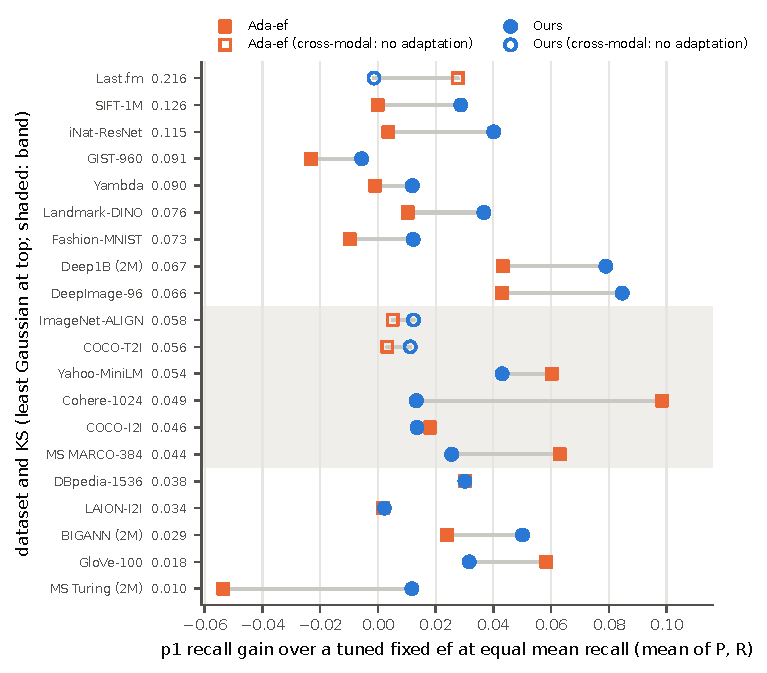
\includegraphics[width=\linewidth]{figures/fig2_p1_vs_ks.pdf}
  \caption{Tail recall gained over a fixed \ef{} at the same mean recall, for Ada-ef and for our
  empirical score, on 20 datasets ordered by how far they are from Gaussian (KS, higher is less
  Gaussian). Above the shaded band, where Ada-ef's Gaussian model does not hold, the empirical score
  wins on every dataset whose queries come from the same modality as the database. Below it, on
  near-Gaussian text embeddings, Ada-ef usually wins. Hollow markers: cross-modal queries, where
  neither score adapts.}
  \label{fig:teaser}
\end{figure}

Graph indexes such as HNSW~\cite{malkov2020hnsw} answer a nearest-neighbor query by a best-first
walk whose breadth is set by one parameter, \ef{}. Most deployments pick one \ef{} for all
queries. That choice is wasteful in both directions: an \ef{} large enough for the hardest queries
spends work on the easy majority, and an \ef{} tuned for the average leaves the hardest queries
short of the recall the application asked for. Several recent systems therefore choose the search
effort per query, either by learning when to stop~\cite{li2020laet,chatzakis2026darth} or by
estimating, before the search, how hard the query will be~\cite{zhang2026adaef}.

Ada-ef~\cite{zhang2026adaef} takes the second route and does so without training a model. It
observes that the similarity between a query $q$ and a random database vector is a sum over many
dimensions, so by the central limit theorem it should be close to Gaussian, with a mean and
variance that follow from the database's mean and covariance. A short probe of the graph then shows
how many of the query's nearby points fall in the extreme tail of that Gaussian, and the count
becomes a difficulty score that maps to an \ef{}. The method is simple and cheap, and on the
OpenAI and Cohere embeddings used in its evaluation it reaches its target recall with up to
4$\times$ lower latency than learned approaches.

The central limit argument, however, is an approximation whose quality depends on the data, and
the Ada-ef paper does not measure it. Neither, as far as we can tell, does any other paper on
nearest-neighbor search: query-hardness measures in the literature
\cite{he2012difficulty,aumuller2019lid,wang2024steiner} either assume such a model or avoid it. We
measured it on 41 datasets from ann-benchmarks, Big-ANN, VIBE and the Ada-ef paper's own sources,
with a Kolmogorov--Smirnov (KS) statistic between each query's actual similarities and the
Gaussian Ada-ef predicts (Fig.~\ref{fig:survey}). Modern contrastive text embeddings fit well. Nine
datasets do not, and they are not exotic: SIFT, GIST, Fashion-MNIST, DeepImage and Deep1B are
among them. Nor does the data type give it away: SIFT-1M is the least Gaussian image dataset we
measured, while SIFT-1B is close to Gaussian, and MNIST fits much better than Fashion-MNIST.

On these datasets Ada-ef's score loses most of its ability to separate easy from hard queries. On
SIFT and on the Yambda audio embeddings it assigns the same \ef{} to every query. We keep Ada-ef's
mechanism (probe, binned score, calibrated \ef{} table) and change one thing: the bin thresholds
come from the data's own distance percentiles instead of from the fitted Gaussian. We call the
result PercEF. It ranks queries better than Ada-ef's on all 8 non-Gaussian datasets we benchmark end to end
and gives better or equal tail recall in all 16 runs (Fig.~\ref{fig:teaser}). It also has a floor
that Ada-ef lacks: across 17 datasets it never costs more than 3.1\% over the best fixed \ef{} at
the same recall, a fixed \ef{} chosen with hindsight on the test queries. Finally, because the
failure is visible in the raw vectors, the same KS statistic tells a practitioner which score to
use before building an index; it picks the better one on 18 of 19 datasets. We also report what
does not work: Ada-ef keeps the better tail on near-Gaussian text embeddings, neither score adapts
when queries come from a different modality than the database, and one prediction (SIFT-1B) fails.

% ------------------------------------------------------------------------------------------------
\section{Related Work}

\paragraph{Adaptive search in graph indexes.}
LAET~\cite{li2020laet} trains a gradient-boosted model on features gathered early in the search to
predict how much longer each query should run. DARTH~\cite{chatzakis2026darth} also terminates
early, but targets a declared recall and checks its prediction periodically during the search.
Both need a training phase with ground truth and adapt the stopping point while the search runs.
Ada-ef~\cite{zhang2026adaef} instead decides \ef{} once, after a short probe, from a statistical
model of the query's similarity distribution; it needs only the database mean and covariance and a
small calibration set, which is what makes it cheap and easy to update. Our method keeps this
design. What we question is the statistical model, which none of these papers test against data.

\paragraph{Query and dataset hardness.}
He et al.~\cite{he2012difficulty} relate the difficulty of nearest-neighbor search to the relative
contrast between nearest and mean distances, derived under a Gaussian-type model of the data.
Aum\"uller and Ceccarello~\cite{aumuller2019lid} show that local intrinsic dimensionality and
related measures vary widely across queries in standard benchmarks and change measured performance.
Hubness~\cite{radovanovic2010hubs} describes how a few points become nearest neighbors of many
queries in high dimensions. Steiner-hardness~\cite{wang2024steiner} measures the effort a graph
index needs for a query from the index itself. These measures describe hardness after the fact or
need the index; none asks whether the distributional model behind a cheap online score holds, which
is the question we answer with a test that runs on the raw vectors.

% ------------------------------------------------------------------------------------------------
\section{Method}

\subsection{Preliminaries}

Let $X \subset \mathbb{R}^d$ be the database, with vectors normalised to unit length so that
cosine similarity and Euclidean distance give the same ranking. For a query $q$ and an integer $k$,
HNSW returns $k$ candidates found by a best-first search whose candidate list holds at most \ef{}
entries; recall@$k$ is the share of the true $k$ nearest neighbors among them. We write
$\mathrm{ef}^*(q)$ for the smallest \ef{} on a grid at which $q$ reaches the target recall $\tau$.

\paragraph{Ada-ef's score.}
Ada-ef models the distance $\delta(q,x) = 1 - q^\top x$ between $q$ and a random database vector
$x$ as
\begin{equation}
  \delta(q,x) \sim \mathcal{N}\!\left(1 - q^\top\mu,\; q^\top \Sigma q\right),
  \label{eq:clt}
\end{equation}
where $\mu$ and $\Sigma$ are the mean and covariance of $X$. It places $B = 5$ thresholds
$t_1 < \dots < t_B$ at the $\beta, 2\beta, \dots, B\beta$ quantiles of this Normal, with
$\beta = 10^{-3}$, so that they mark the closest tenth of a percent of the database, the next
tenth, and so on. An unpruned best-first probe collects the first $L = 1025$ distances the search
meets, $P(q)$, and the score is
\begin{equation}
  s(q) = \frac{1}{|P(q)|} \sum_{p \in P(q)} w_{b(p)}, \qquad w_b = 100\, e^{-(b-1)},
  \label{eq:score}
\end{equation}
where $b(p)$ is the first bin whose threshold $p$ falls below (points beyond $t_B$ add nothing). A
query surrounded by many unusually close points scores high and is easy; a query whose probe finds
few is hard. Offline, Ada-ef scores a calibration set, groups it by rounded score, and stores for
each group the smallest \ef{} at which the group's average recall reaches $\tau$. Its paper also
floors every entry at the weighted average of these values (WAE); the released code does not. We
report both variants.

\subsection{Testing the Gaussian assumption}

Equation~\eqref{eq:clt} can be checked directly. For a query $q$ we compute the similarities
$q^\top x$ to a uniform sample of the database and the KS statistic between their empirical
distribution and the Normal implied by~\eqref{eq:clt},
\begin{equation}
  \KS(q) = \sup_z \left| \hat F_q(z) - \Phi\!\left(\frac{z - q^\top\mu}{\sqrt{q^\top\Sigma q}}\right) \right| .
\end{equation}
We report the mean over 200 test queries, with $\mu$ and $\Sigma$ estimated from up to $10^6$
database vectors and $\KS(q)$ from 20{,}000. With 30 queries the estimate was noisy by as much as
the effects we were trying to see, which is why we use 200 and report a 95\% interval. The test
needs only the vectors and a few seconds per dataset.

\subsection{PercEF: an empirical difficulty score}

The thresholds in~\eqref{eq:score} are the only place where the Gaussian enters Ada-ef's score.
We take them from the data instead. Let $c_1,\dots,c_C$ be centroids of $X$ ($C = 1$ gives the
database mean) and, for each centroid, let $t^{(c)}_b$ be the empirical $b\beta$ quantile of the
squared distances $\lVert x - c \rVert^2$ of the database vectors assigned to it. At query time we
find the nearest centroid, probe the first $L = 100$ distances, and evaluate~\eqref{eq:score} with
these thresholds and the same weights. The thresholds thus describe what ``unusually close'' means
in this particular database, whatever the shape of its distance distribution.

For calibration we measure $\mathrm{ef}^*(q)$ for every calibration query and fit an isotonic
regression~\cite{barlow1972isotonic} of $\mathrm{ef}^*$ on the rounded score, letting the fit
choose the direction, and clip the result to $[k, 5000]$. The search does not restart after the
probe: it continues the same traversal with the chosen \ef{}, so the probe's distance computations
are part of the search, not an addition to it. Our default, fixed before the end-to-end runs, is
$C = 1$ with isotonic calibration; we also ran $C \in \{8, 50\}$ and three bucket recipes and treat
them as secondary.

The two scores differ in their thresholds, in the probe length (100 against 1025) and in how the
\ef{} table is built. The rank correlation we report between score and $\mathrm{ef}^*$ depends only
on the first two. Ada-ef's longer probe gives its score more information, not less, so we do not
expect the difference in probe length to favour us; we did not run a version of Ada-ef with a
shorter probe.

\subsection{Implementation}

Both methods run inside the same HNSWlib build. Ada-ef runs through its authors' own code: we call
their scoring, sketch and search routines unchanged and only add a loader that reads the database
statistics from a file, so that they can be computed in one streaming pass. On every dataset that
fits in memory we also built Ada-ef's estimator the original way and checked that the two give the
same scores (50 of 50 queries identical on all of them). Our score is computed inside the same
traversal, with the same memory prefetching as HNSWlib's own search loop. All searches run on one
thread.

% ------------------------------------------------------------------------------------------------
\section{Experiments}

\subsection{Setup}

\paragraph{Datasets.}
We benchmark 20 datasets end to end (Table~\ref{tab:datasets}): the four in the Ada-ef paper that
we could obtain (GloVe-100, DeepImage-96, Cohere-1024 and LAION-I2I, the last two as subsets that
fit in 62\,GB of memory), a MiniLM-384 stand-in for its MS MARCO set, standard ann-benchmarks sets
\cite{aumuller2020annbenchmarks}, 2M-vector prefixes of three Big-ANN sets~\cite{simhadri2022bigann}
(the benchmark builds its own subsets the same way), four VIBE sets~\cite{jaasaari2025vibe}, and
Yambda audio embeddings~\cite{ploshkin2025yambda}. Fourteen of them were added after the first six,
each with its outcome predicted in advance from KS (\S\ref{sec:predict}). Three have queries from a
different modality than the database (text against images, users against songs).

\paragraph{Protocol.}
We follow the Ada-ef paper: HNSW with $M = 16$ and $\mathit{ef}_{\mathrm{construction}} = 500$,
$k = 1000$ for the MS MARCO, Cohere and LAION sets and $k = 100$ otherwise, target recall
$\tau = 0.95$, and \ef{} capped at 5000. Both methods always calibrate on the same set, in two
settings: \emph{P}, 200 database vectors as in the Ada-ef paper, and \emph{R}, up to 2000 held-out
real queries. Test queries are disjoint from both.

\paragraph{Metrics and the fixed-\ef{} reference.}
We report what the Ada-ef paper reports: mean recall against the target, tail recall (the 1st and
5th percentile of per-query recall, p1 and p5), latency per query, and offline cost. Distance
computations (DC), including every probe, serve as a hardware-independent measure of cost. As a
reference we run HNSW at a grid of fixed \ef{} values and, for each method, interpolate the fixed
\ef{} that reaches the same mean recall. This is the best fixed \ef{} anyone could choose in
hindsight; no deployment can pick it in advance, so beating it is a demanding test, and it is not a
claim the Ada-ef paper makes. We interpolate in $\log(1 - \text{recall})$ against $\log$ cost:
interpolating linearly overstates the fixed \ef{}'s cost by 11\% on average in a leave-one-out
test on our grids (\S\ref{sec:pitfalls}), which would flatter every adaptive method.

\begin{table}[t]
  \caption{Datasets, sorted by KS (200 queries). $\rho$: rank correlation between each score and
  the true per-query $\mathrm{ef}^*$ on the calibration set, settings P / R; the larger magnitude
  ranks queries better. A dash: the score is constant on the calibration queries.}
  \label{tab:datasets}
  \centering\footnotesize
  \resizebox{\linewidth}{!}{\begin{tabular}{lllrrrrrrrrr}
\toprule
dataset & source & in Ada-ef paper & corpus & dim & K & test queries & KS & rho Ada-ef P & rho ours P & rho Ada-ef R & rho ours R \\
\midrule
MS Turing (2M) & Big-ANN & no & 2,000,000 & 100 & 100 & 10000 & 0.010 & -0.36 & -0.35 & -0.48 & -0.40 \\
GloVe-100 & ann-benchmarks & yes & 1,183,514 & 100 & 100 & 8000 & 0.018 & -0.81 & -0.61 & -0.80 & -0.61 \\
BIGANN (2M) & Big-ANN & no & 2,000,000 & 128 & 100 & 8000 & 0.029 & -0.42 & -0.74 & -0.42 & -0.74 \\
LAION-I2I & LAION, shards 0-19 & yes (subset) & 19,639,187 & 512 & 1000 & 10000 & 0.034 & -0.59 & -0.56 & -0.57 & -0.53 \\
DBpedia-1536 & DBpedia, OpenAI embeddings & no & 990,000 & 1536 & 100 & 8000 & 0.038 & -0.48 & -0.38 & -0.48 & -0.54 \\
MS MARCO-384 & MS MARCO (MiniLM) & stand-in & 8,841,823 & 384 & 1000 & 6980 & 0.044 & -0.66 & -0.53 & -0.69 & -0.53 \\
COCO-I2I & ann-benchmarks & no & 113,287 & 512 & 100 & 8000 & 0.046 & -0.33 & -0.39 & -0.35 & -0.36 \\
Cohere-1024 & Cohere, files 00-04 & yes (subset) & 9,511,868 & 1024 & 1000 & 1174 & 0.049 & -0.59 & -0.40 & -0.79 & -0.52 \\
Yahoo-MiniLM & VIBE & no & 677,305 & 384 & 100 & 700 & 0.054 & -0.55 & -0.54 & -0.50 & -0.68 \\
COCO-T2I & ann-benchmarks & no & 113,287 & 512 & 100 & 8000 & 0.056 & -0.34 & -0.38 & -- & -- \\
ImageNet-ALIGN & VIBE & no & 1,281,167 & 640 & 100 & 1000 & 0.058 & -0.17 & -0.23 & -- & -- \\
DeepImage-96 & ann-benchmarks & yes & 9,990,000 & 96 & 100 & 8000 & 0.066 & -0.42 & -0.63 & -0.38 & -0.62 \\
Deep1B (2M) & Big-ANN & no & 2,000,000 & 96 & 100 & 8000 & 0.067 & -0.39 & -0.64 & -0.41 & -0.67 \\
Fashion-MNIST & ann-benchmarks & no & 60,000 & 784 & 100 & 8000 & 0.073 & -0.20 & -0.22 & -0.17 & -0.29 \\
Landmark-DINO & VIBE & no & 760,757 & 768 & 100 & 700 & 0.076 & -0.45 & -0.61 & -0.34 & -0.55 \\
Yambda & Yambda & no & 7,709,749 & 128 & 100 & 10000 & 0.090 & +0.02 & -0.41 & -0.03 & -0.43 \\
GIST-960 & ann-benchmarks & no & 1,000,000 & 960 & 100 & 700 & 0.091 & -0.10 & -0.46 & +0.08 & -0.23 \\
iNat-ResNet & VIBE & no & 499,000 & 2048 & 100 & 700 & 0.115 & -0.24 & -0.46 & -0.21 & -0.46 \\
SIFT-1M & ann-benchmarks & no & 1,000,000 & 128 & 100 & 8000 & 0.126 & +0.08 & -0.33 & -0.04 & -0.45 \\
Last.fm & ann-benchmarks & no & 292,385 & 65 & 100 & 10000 & 0.216 & +0.07 & +0.23 & -- & -- \\
\bottomrule
\end{tabular}
}
\end{table}

\subsection{How often does the assumption hold?}

Figure~\ref{fig:survey} shows KS for all 41 datasets. Most lie below 0.044, the level up to which
Ada-ef's score ranked queries better than ours in our runs. They are mostly text and text-image
embeddings (OpenAI, Cohere, MiniLM, Nomic, CLIP and others), but word vectors, LLM attention keys
and SIFT-1B are among them too. Nine lie at or above the band's upper edge, set by DeepImage at
0.066: SIFT-1M, GIST, Fashion-MNIST, DeepImage, Deep1B, iNaturalist ResNet, Landmark DINO, Yambda
and Last.fm. Between the two is a band where neither wins clearly.
Datasets built from the same kind of data land on different sides (SIFT-1M at 0.126, SIFT-1B at
0.029; Fashion-MNIST at 0.073, MNIST at 0.037), so the assumption has to be checked on the data
itself.

\begin{figure}[t]
  \centering
  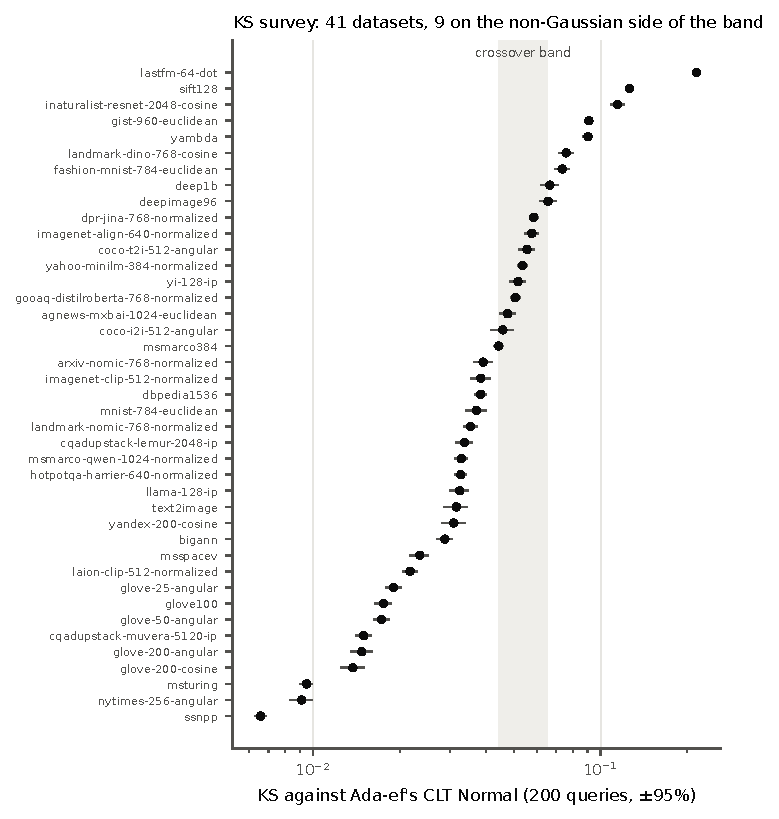
\includegraphics[width=0.92\linewidth]{figures/fig1_ks_survey.pdf}
  \caption{KS between each query's similarities and Ada-ef's Gaussian, mean over 200 queries with
  95\% interval, for 41 public datasets. Shaded: the band in which neither score ranks queries
  clearly better. GloVe-200 appears twice, from ann-benchmarks and from VIBE.}
  \label{fig:survey}
\end{figure}

\subsection{Comparison on non-Gaussian datasets}

Table~\ref{tab:counts} summarises every run against the fixed-\ef{} reference, and
Fig.~\ref{fig:cost} shows where each method sits relative to the fixed-\ef{} curve. On the eight
datasets above the band (16 runs), our score has the larger rank correlation with $\mathrm{ef}^*$
in all 16 and a tail gain at least as large as Ada-ef's in all 16. The gains are often large: p1
rises by 0.086 over the fixed \ef{} on DeepImage (Ada-ef 0.045), by 0.079 on Deep1B (0.044) and
by 0.040 on iNaturalist (0.004). Ada-ef costs more than the fixed \ef{} in 14 of these 16 runs; ours
costs less in 14, and the two exceptions are small (DeepImage P, 3.1\% more; GIST R, 1.0\% more).

On SIFT-1M and Yambda, Ada-ef's score collapses: every query lands in the same group and gets the
same \ef{}. Ada-ef then behaves as a fixed \ef{} that also pays for a 1025-distance probe. Ours
still separates queries, with rank correlations of 0.33 to 0.45 against $\mathrm{ef}^*$. The gains
are not uniform. On GIST both scores do little for the tail (ours $-$0.006, Ada-ef $-$0.023), and
on Fashion-MNIST most queries reach the target at the smallest \ef{}, which leaves little room for
any adaptive method.

\begin{table}[t]
  \caption{Runs in which each method is cheaper than the fixed \ef{} at the same mean recall (DC),
  faster (latency; measured on 8 adaptive runs so far), and has at least its p1 tail recall. Same
  modality unless marked. Worst: the largest extra cost.}
  \label{tab:counts}
  \centering\footnotesize
  \begin{tabular}{llrrrr}
    \toprule
    Datasets & Method & Cheaper & Worst & Faster & p1 $\geq$ \\
    \midrule
    All (34 runs)        & Ours        & 32/34 & $-$3.1\%  & 6/8 & 33/34 \\
                         & Ada-ef      & 11/34 & $-$23.9\% & 0/8 & 24/34 \\
                         & Ada-ef WAE  & 17/34 & $-$23.9\% & 1/8 & 25/34 \\
    \midrule
    KS $\geq$ 0.066 (16) & Ours        & 14/16 & $-$3.1\%  & 0/2 & 15/16 \\
                         & Ada-ef      &  2/16 & $-$23.9\% & 0/2 &  8/16 \\
    Band (8)             & Ours        &   8/8 & $+$3.0\%  & 2/2 &   8/8 \\
                         & Ada-ef      &   5/8 & $-$7.4\%  & 0/2 &   8/8 \\
    KS $<$ 0.044 (10)    & Ours        & 10/10 & $+$1.9\%  & 4/4 & 10/10 \\
                         & Ada-ef      &  4/10 & $-$12.3\% & 0/4 &  8/10 \\
                         & Ada-ef WAE  &  8/10 & $-$2.0\%  & 1/4 &  8/10 \\
    \midrule
    Cross-modal (6)      & Ours        &   1/6 & $-$1.3\%  & 0/4 &   5/6 \\
                         & Ada-ef      &   0/6 & $-$10.3\% & 0/4 &   4/6 \\
    \bottomrule
  \end{tabular}
\end{table}

\begin{figure*}[t]
  \centering
  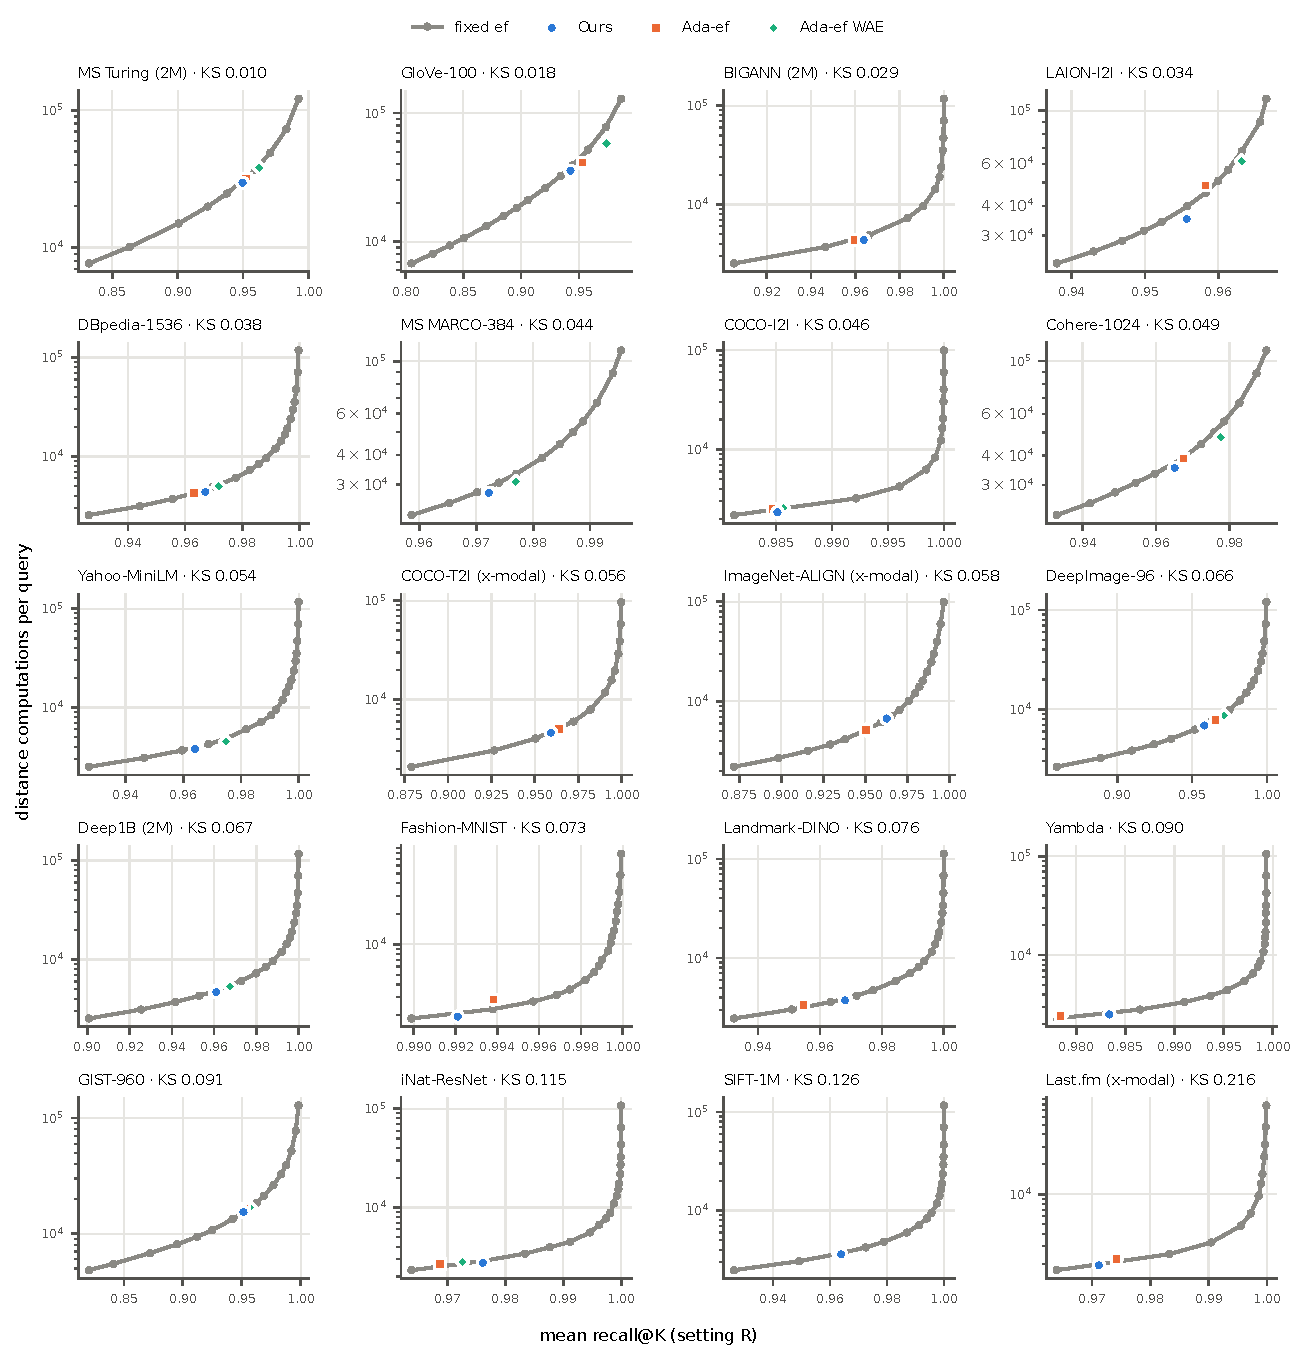
\includegraphics[width=0.95\textwidth]{figures/fig3_cost_vs_recall.pdf}
  \caption{Distance computations per query against mean recall, setting R. Grey: HNSW with fixed
  \ef{}. Points below the curve reach the same recall with less work. Panels are ordered by KS, from
  near-Gaussian (top left) to non-Gaussian (bottom right).}
  \label{fig:cost}
\end{figure*}

\subsection{Comparison on near-Gaussian datasets}

Below the band the picture reverses. Ada-ef's score ranks queries better on GloVe, MS MARCO and
Cohere, and its tail is better: p1 gains of 0.058, 0.063 and 0.099 over the fixed \ef{}, against
our 0.031, 0.025 and 0.014. With its WAE floor it is also cheaper than the fixed \ef{} by a wide
margin on these sets (27\% on GloVe, 7\% on MS MARCO, 4--11\% on Cohere and LAION). Ours stays
cheaper than the fixed \ef{} on all of them, but gives a smaller tail gain. We therefore do not
claim that the empirical score should replace Ada-ef's. On text embeddings like those in the
Ada-ef paper, the Gaussian model is a good one and Ada-ef uses it well.

Two datasets on this side behave differently. On SIFT-1B (KS 0.029) our score ranks queries far
better (0.74 against 0.42) and has the better tail. On MS Turing (KS 0.010) Ada-ef ranks better, as
expected, yet its tail is worse than the fixed \ef{}'s (p1 $-$0.067 and $-$0.041) because its
group-average table under-provisions some score groups; with the WAE floor it is level.

\subsection{Analysis}

\paragraph{Predicting the better score.}\label{sec:predict}
Across datasets, KS correlates with Ada-ef's rank correlation at $-0.87$ (13 datasets, setting R).
To use it as a rule, we set the band from the first six datasets and wrote down a prediction for
each of the other fourteen before running it. It held for Landmark-DINO, iNaturalist, GIST,
Fashion-MNIST and Deep1B on our side, and for LAION, Cohere and MS Turing on Ada-ef's; Yahoo-MiniLM
and COCO-I2I fell in the band as predicted and split or tied; three cross-modal sets could not be
scored (below); and SIFT-1B failed. Over the 19 datasets with a clear winner, a single KS threshold
sorts 18 correctly, and 16 when each threshold is fitted without the dataset it predicts.

We expected the SIFT-1B failure to come from the tail: Ada-ef's thresholds sit at the 0.1\%
quantiles, where KS, dominated by the bulk of the distribution, says little. So we measured the tail
directly, with Anderson--Darling~\cite{anderson1952}, the error of the Normal's upper quantiles, and
the mass beyond its 99.9\% point (Table~\ref{tab:tail} in the appendix). None did better than
always predicting our score, and the reason is in the numbers: the text embeddings on which Ada-ef
wins have the least Gaussian upper tails (MS MARCO $+$2.3 standard deviations at the $10^{-4}$
quantile), while SIFT-1B's tail is close to Gaussian. How well the Normal fits the tail is not what
decides whether the score works, and we do not yet know what makes SIFT-1B different. A cheap
check covers the case in practice: Ada-ef's calibration already scores a few hundred points, and
when those scores take only a handful of distinct values (5 to 11 on SIFT-1B, against 60 to 100 on
datasets where the score works), the score cannot rank queries.

\paragraph{Latency and offline cost.}
On the six datasets timed so far, all with $k = 100$, our method is between 2.9\% slower and
2.5\% faster than the fixed \ef{} at the same recall. It saves fewer microseconds than distance
computations because its per-query overhead (the probe phase, scoring and the table lookup) does
not shrink with the query. Ada-ef is slower than the fixed \ef{} on all of them, by up to 39\%,
and by 87\% on Last.fm, where a whole search takes 0.13\,ms and its 1025-distance probe dominates.
With $k = 100$ and small \ef{} this is Ada-ef's least favourable regime; on its own datasets, with
$k = 1000$, the probe is a small part of a much longer search
\pending{latency on GloVe, DeepImage, MS MARCO, Cohere, LAION: measuring}. Offline, both
methods need seconds for their statistics. Calibration time is dominated by measuring
$\mathrm{ef}^*$ (ours, up to 257\,s on MS Turing) and by Ada-ef's per-group search (206\,s on the
same set). Ada-ef keeps a $d \times d$ covariance (up to 9.4\,MB at $d = 1536$); ours keeps five
thresholds, the centroid and the table, a few kilobytes.

\paragraph{Cross-modal queries.}
On Last.fm (user vectors against song vectors), COCO text-to-image and ImageNet ALIGN text-to-image,
both scores are constant on real queries: every query gets the same \ef{}. Real queries lie far
from every database vector, so no probe distance reaches the region either score distinguishes.
This is a limitation of both methods. Ours then behaves as a fixed \ef{} at about the right value
(between 1.3\% more and 0.5\% less work); Ada-ef also pays for its probe, up to 10\% more work and
87\% more time.

\paragraph{Controlled data.}
Varying the distribution of synthetic data moves the ranking advantage in the expected direction
in most but not all runs (Fig.~\ref{fig:controlled} in the appendix); one cluster-separation run at
KS 0.10 favours Ada-ef. We treat it as supporting evidence, not as proof.

\subsection{Pitfalls in evaluating adaptive search}\label{sec:pitfalls}

Several of our own intermediate results did not survive closer measurement, and the reasons apply
to any adaptive-\ef{} method. Interpolating the fixed-\ef{} reference linearly between grid points
credited every method with 3--4\% of savings it did not have; we found it because two methods that
assign one \ef{} to every query were credited with savings over a fixed \ef{}. Timing each method
once, in sequence, made latency vary by 24\% between identical runs; we time in three rounds with
the method order rotated and take per-query medians. KS from 30 queries was noisy by as much as the
width of the band. Probe cost must be counted: Ada-ef's fixed probe is a large share of a short
search. And about 2\% of LAION queries cannot reach the target at any \ef{} up to the cap, which
limits every method's p1 there; we report LAION's tail at p5.

% ------------------------------------------------------------------------------------------------
\section{Conclusion}

Ada-ef chooses the search breadth of each HNSW query from a Gaussian model of its similarities. We
measured that model on 41 datasets and found it holds for most modern text embeddings and fails on
nine, which cannot be told apart by data type. Where it fails, PercEF, which replaces the Gaussian
thresholds with the data's own percentiles, restores the score's ability to rank queries and gives better tail
recall in every run, at a cost that never exceeds a hindsight-tuned fixed \ef{} by more than 3.1\%.
A KS test on the raw vectors tells which score to use before an index is built, with one known
miss. Neither score adapts when queries come from another modality, and on near-Gaussian data
Ada-ef's remains the better choice. Code, data pointers and every number in this paper are
generated from the released result files. \pending{repository URL}

\bibliographystyle{ACM-Reference-Format}
\bibliography{refs}

% ------------------------------------------------------------------------------------------------
\appendix
\section{Additional results}

\begin{figure}[h]
  \centering
  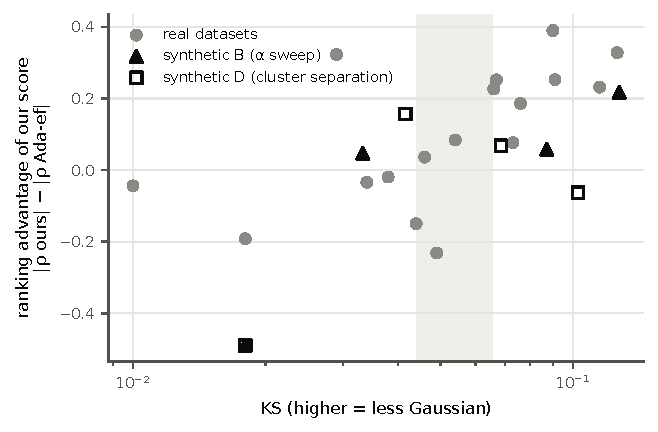
\includegraphics[width=\linewidth]{figures/fig4_controlled.pdf}
  \caption{Ranking advantage of the empirical score against KS for the real datasets and for
  synthetic data with controlled anisotropy (B) and cluster separation (D).}
  \label{fig:controlled}
\end{figure}

\begin{figure}[h]
  \centering
  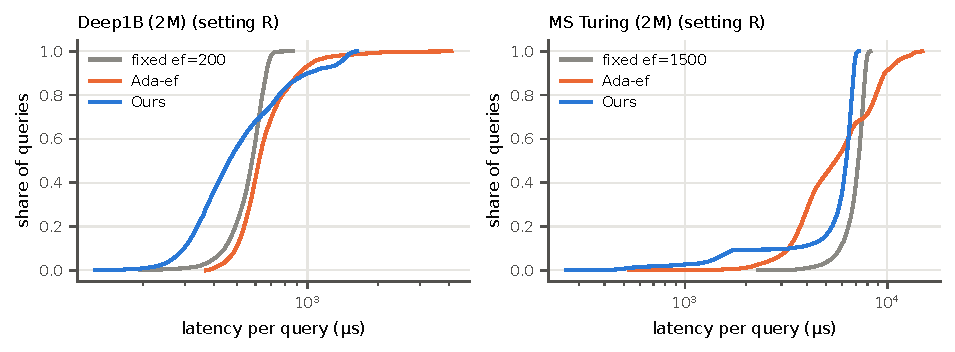
\includegraphics[width=\linewidth]{figures/fig3c_latency_cdf.pdf}
  \caption{Per-query latency on Deep1B and MS Turing (setting R). The empirical score spends less
  time on easy queries and more on hard ones; a fixed \ef{} spends about the same on all.}
  \label{fig:cdf}
\end{figure}

\begin{table*}[h]
  \caption{Tail-weighted alternatives to KS on the raw vectors. Tail $z$: distance of the
  empirical upper quantile from the Normal's, in standard deviations. Tail mass: $\log_{10}$ of
  the observed over the expected share beyond the Normal's 99.9\% point. Margin:
  $|\rho_{\text{ours}}| - |\rho_{\text{Ada-ef}}|$, mean over P and R.}
  \label{tab:tail}
  \centering\footnotesize
  \begin{tabular}{llrrrrrrr}
\toprule
dataset & source & KS & AD/n & tail z 1e-2 & tail z 1e-3 & tail z 1e-4 & tail mass 99.9\% & rho margin \\
\midrule
MS Turing (2M) & Big-ANN & 0.0090 & 0.0001 & -0.02 & -0.02 & +0.04 & -0.11 & -0.044 \\
GloVe-100 & ann-benchmarks & 0.0167 & 0.0005 & -0.04 & +0.04 & +0.12 & -0.12 & -0.192 \\
BIGANN (2M) & Big-ANN & 0.0299 & 0.0015 & +0.08 & -0.05 & -0.26 & -0.27 & +0.323 \\
LAION-I2I & LAION, shards 0-19 & 0.0328 & 0.0020 & -0.09 & +0.02 & +0.06 & -0.36 & -0.034 \\
DBpedia-1536 & DBpedia, OpenAI embeddings & 0.0387 & 0.0034 & +0.31 & +0.93 & +1.49 & +0.60 & -0.019 \\
MS MARCO-384 & MS MARCO (MiniLM) & 0.0444 & 0.0044 & +0.57 & +1.36 & +2.29 & +0.85 & -0.150 \\
Cohere-1024 & Cohere, files 00-04 & 0.0452 & 0.0045 & +0.52 & +1.19 & +1.91 & +0.80 & -0.232 \\
COCO-I2I & ann-benchmarks & 0.0458 & 0.0026 & +0.51 & +0.76 & +0.75 & +0.69 & +0.036 \\
Yahoo-MiniLM & VIBE & 0.0543 & 0.0064 & +0.67 & +1.43 & +2.12 & +0.90 & +0.084 \\
COCO-T2I & ann-benchmarks & 0.0563 & 0.0067 & +0.75 & +1.05 & +1.09 & +0.94 & +0.035 \\
ImageNet-ALIGN & VIBE & 0.0566 & 0.0062 & +0.77 & +2.20 & +3.18 & +0.98 & +0.054 \\
DeepImage-96 & ann-benchmarks & 0.0656 & 0.0085 & +0.57 & +0.76 & +0.75 & +0.69 & +0.226 \\
Deep1B (2M) & Big-ANN & 0.0674 & 0.0075 & +0.61 & +0.77 & +0.75 & +0.69 & +0.252 \\
Fashion-MNIST & ann-benchmarks & 0.0711 & 0.0074 & -0.38 & -0.89 & -1.38 & -1.88 & +0.077 \\
Landmark-DINO & VIBE & 0.0750 & 0.0121 & +0.66 & +1.09 & +1.31 & +0.81 & +0.186 \\
Yambda & Yambda & 0.0902 & 0.0174 & +1.03 & +1.54 & +1.50 & +1.10 & +0.390 \\
GIST-960 & ann-benchmarks & 0.0913 & 0.0213 & -0.78 & -1.24 & -1.64 & -2.55 & +0.253 \\
iNat-ResNet & VIBE & 0.1128 & 0.0248 & +0.94 & +1.70 & +2.02 & +0.74 & +0.232 \\
SIFT-1M & ann-benchmarks & 0.1278 & 0.0301 & -0.48 & -0.97 & -1.43 & -3.13 & +0.328 \\
Last.fm & ann-benchmarks & 0.2150 & 0.0918 & +1.64 & +7.25 & +11.05 & +1.17 & +0.162 \\
\bottomrule
\end{tabular}

\end{table*}

\begin{table*}[h]
  \caption{Offline cost, round-2 datasets.}
  \centering\footnotesize
  \begin{tabular}{llrrrrrr}
\toprule
dataset & setting & Ada-ef statistics (s) & Ada-ef table (s) & Ada-ef memory (B) & ours bins (s) & ours min-ef (s) & ours memory (B) \\
\midrule
MS Turing (2M) & P & 5.2 & 5.1 & 41,320 & 0.7 & 7.4 & 824 \\
MS Turing (2M) & R & 5.2 & 206.2 & 41,528 & 0.7 & 257.5 & 768 \\
BIGANN (2M) & P & 4.8 & 0.3 & 66,600 & 0.8 & 0.3 & 936 \\
BIGANN (2M) & R & 4.8 & 3.0 & 66,648 & 0.8 & 3.3 & 936 \\
COCO-I2I & P & 1.7 & 0.1 & 1,053,160 & 0.2 & 0.1 & 2,472 \\
COCO-I2I & R & 1.7 & 1.0 & 1,053,472 & 0.2 & 1.1 & 2,472 \\
COCO-T2I & P & 1.7 & 0.1 & 1,053,176 & 0.2 & 0.1 & 2,472 \\
COCO-T2I & R & 1.7 & 8.0 & 1,052,680 & 0.2 & 9.7 & 2,072 \\
Deep1B (2M) & P & 5.8 & 0.2 & 37,800 & 0.6 & 0.2 & 808 \\
Deep1B (2M) & R & 5.8 & 3.0 & 38,072 & 0.6 & 3.3 & 808 \\
Last.fm & P & 0.8 & 0.4 & 17,436 & 0.1 & 2.1 & 684 \\
Last.fm & R & 0.8 & 0.3 & 17,428 & 0.1 & 0.4 & 284 \\
\bottomrule
\end{tabular}

\end{table*}

\end{document}
